\chapter{DASAR TEORI}

\section{Variabel Random}
\label{sec:variabelrandom}

Variabel random memetakan setiap hasil suatu percobaan acak ke sebuah bilangan
real sehingga hasil percobaan dapat diperlakukan secara kuantitatif.

\begin{definisi}[\citealp{bain}]
\label{def:varrandom}
\textit{Variabel random} $X$ adalah fungsi dengan daerah asal ruang sampel $S$
yang memetakan setiap anggota $S$ ke bilangan real,
\begin{equation*}
  X:\; S\longrightarrow\mathbb{R},\qquad X(e)=x,\quad e\in S,\; x\in\mathbb{R}.
  \label{eq:varrandom}
\end{equation*}
\end{definisi}

Variabel random dinotasikan dengan huruf kapital $X$, $Y$, $Z$, sedangkan nilai
yang mungkin diambil dinotasikan dengan huruf kecil $x$, $y$, $z$.
Berdasarkan himpunan nilai yang mungkin diambil, variabel random dibedakan
menjadi diskret dan kontinu.

\subsection{Variabel Random Diskret dan Kontinu}
\label{subsec:jenisvariabelrandom}

Variabel random dibedakan menjadi variabel random diskret dan kontinu
berdasarkan himpunan nilai yang mungkin diambil serta cara distribusi
probabilitasnya dinyatakan.

\begin{definisi}[\citealp{bain}]
\label{def:vardiskret}
Variabel random $X$ disebut \textit{diskret} apabila himpunan semua nilai
yang mungkin diambil, $\{x_1,x_2,x_3,\ldots\}$, merupakan himpunan
terhitung (\textit{countable}).
\end{definisi}

Untuk variabel random diskret, distribusi probabilitas dinyatakan melalui
fungsi massa peluang (\textit{probability mass function}, pmf).

\begin{definisi}[\citealp{bain}]
\label{def:pmfdiskret}
Fungsi massa peluang dari variabel random diskret $X$ adalah fungsi
$p_X$ yang didefinisikan sebagai
\begin{equation}
    p_X(x)=P(X=x),\qquad x\in\mathcal{X},
    \label{eq:pmfdiskret}
\end{equation}
dengan $\mathcal{X}$ merupakan himpunan nilai yang mungkin diambil oleh
$X$. Fungsi tersebut memenuhi
\begin{equation}
    p_X(x)\geq 0,\qquad
    \sum_{x\in\mathcal{X}}p_X(x)=1.
    \label{eq:syaratpmfdiskret}
\end{equation}
\end{definisi}

Sementara itu, variabel random kontinu didefinisikan melalui fungsi
distribusi kumulatifnya yang dapat dinyatakan sebagai integral suatu
fungsi kepadatan peluang.

\begin{definisi}[\citealp{bain}]
\label{def:varkontinu}
Variabel random $X$ disebut \textit{kontinu} apabila terdapat fungsi
$f_X$, yang disebut \textit{fungsi kepadatan peluang}
(\textit{probability density function}, pdf), sedemikian sehingga
fungsi distribusi kumulatifnya memenuhi
\begin{equation}
    F_X(x)=\int_{-\infty}^{x}f_X(t)\,dt,
    \qquad x\in\mathbb{R}.
    \label{eq:cdfkontinu}
\end{equation}
\end{definisi}

\begin{definisi}[\citealp{bain}]
\label{def:pdfkontinu}
Fungsi $f_X$ merupakan fungsi kepadatan peluang dari variabel random
kontinu $X$ jika memenuhi
\begin{equation}
    f_X(x)\geq 0,\qquad x\in\mathbb{R},
    \label{eq:nonnegatifpdf}
\end{equation}
dan
\begin{equation}
    \int_{-\infty}^{\infty}f_X(x)\,dx=1.
    \label{eq:syaratpdf}
\end{equation}
Peluang bahwa $X$ berada pada interval $[a,b]$, dengan $a\leq b$,
diperoleh melalui
\begin{equation}
    P(a\leq X\leq b)=\int_a^b f_X(x)\,dx.
    \label{eq:peluangintervalkontinu}
\end{equation}
\end{definisi}


\section{Ekspektasi dan Variansi}

\label{sec:ekspektasi}

\subsection{Ekspektasi Variabel Random}

\label{subsec:hargaharapan}

Ekspektasi merupakan salah satu ukuran yang digunakan untuk menunjukkan nilai
rata-rata yang diharapkan dari suatu variabel random. Untuk variabel random
diskret, ekspektasi diperoleh melalui penjumlahan nilai-nilai yang mungkin,
sedangkan untuk variabel random kontinu digunakan integral.

\begin{definisi}[\citealp{subanar}]

\label{def:hargaharapan}

Ekspektasi atau \textit{expected value} dari variabel random $X$ dapat ditulis
sebagai

\begin{equation}
\mathbb{E}[X]=
\begin{cases}
\displaystyle\sum_x x f(x), & X \text{ diskret dengan pmf } f,\\[1.2ex]
\displaystyle\int_{-\infty}^{\infty}x f(x)\,dx,
& X \text{ kontinu dengan pdf } f.
\end{cases}
\label{eq:hargaharapan}
\end{equation}

dengan syarat jumlahan atau integral tersebut konvergen. Ekspektasi
$\mathbb{E}[X]$ juga biasa dinotasikan dengan $\mu$ atau $\mu_X$.

\end{definisi}

Untuk fungsi dari suatu variabel random, ekspektasi dapat diperoleh dengan
menggantikan $x$ pada Persamaan~\eqref{eq:hargaharapan} dengan fungsi tersebut.

\begin{definisi}[\citealp{bain}]

\label{teo:ekspektasifungsi}

Jika $u$ merupakan fungsi bernilai real dari variabel random $X$, maka

\begin{equation}
\mathbb{E}[u(X)]=
\begin{cases}
\displaystyle\sum_x u(x)f(x), & X \text{ diskret},\\[1.2ex]
\displaystyle\int_{-\infty}^{\infty}u(x)f(x)\,dx,
& X \text{ kontinu}.
\end{cases}
\label{eq:ekspektasifungsi}
\end{equation}

\end{definisi}

Salah satu sifat penting dari ekspektasi adalah sifat linearitas. Jika terdapat
dua fungsi dari variabel random yang dikalikan dengan suatu konstanta, maka
ekspektasinya dapat dihitung secara terpisah.

\subsection{Ekspektasi Vektor Random}

\label{subsec:ekspektasivektor}

Ekspektasi suatu vektor random diperoleh dengan menghitung ekspektasi dari setiap komponennya. 
Setiap komponen pada vektor ekspektasi menyatakan nilai harapan dari komponen 
vektor random yang bersesuaian. Sehingga untuk vektor random $\bm{X}$,
Ekspektasinya adalah

\begin{equation}
\mathbb{E}[\bm{X}]
=
\bigl(
\mathbb{E}[X_1],\dots,\mathbb{E}[X_p]
\bigr)^{\top}
\in\mathbb{R}^{p}.
\label{eq:ekspektasivektor}
\end{equation}

Jika $\bm{u}(X)=(u_1(X),\dots,u_p(X))^\top$, maka ekspektasi juga dapat
diterapkan pada setiap komponen sehingga

\begin{equation}
\mathbb{E}[\bm{u}(X)]
=
\begin{cases}
\displaystyle\sum_x \bm{u}(x)f(x), & X \text{ diskret},\\[1.2ex]
\displaystyle\int_{-\infty}^{\infty}
\bm{u}(x)f(x)\,dx, & X \text{ kontinu}.
\end{cases}
\label{eq:ekspektasivektorfungsi}
\end{equation}

Hasil dari Persamaan~\eqref{eq:ekspektasivektorfungsi} merupakan sebuah
vektor yang berada di $\mathbb{R}^p$.

\subsection{Variansi dan Kovariansi}
\label{subsec:variansi}

Variansi mengukur seberapa besar penyebaran nilai suatu variabel random terhadap nilai harapannya. Variansi yang kecil menunjukkan bahwa nilai variabel cenderung berada dekat dengan nilai harapannya, sedangkan variansi yang besar menunjukkan penyebaran yang lebih luas.

\begin{definisi}[\citealp{bain}]
\label{def:variansi}

Variansi variabel random \(X\) didefinisikan sebagai
\begin{equation}
\operatorname{Var}(X)
=
\mathbb{E}\left[(X-\mathbb{E}[X])^2\right].
\label{eq:variansi}
\end{equation}

Variansi juga dapat dinotasikan dengan \(\sigma^2\) atau \(\sigma_X^2\).
Akar kuadrat dari variansi disebut standar deviasi, yaitu
\begin{equation}
\sigma=\sqrt{\operatorname{Var}(X)}.
\label{eq:standardeviasi}
\end{equation}
\end{definisi}

Kovariansi mengukur kecenderungan dua variabel random berubah bersama. Kovariansi positif menunjukkan kecenderungan perubahan searah, sedangkan kovariansi negatif menunjukkan kecenderungan perubahan berlawanan arah. Kovariansi antara \(X\) dan \(Y\) didefinisikan sebagai
\begin{equation}
\operatorname{Cov}(X,Y)
=
\mathbb{E}\left[(X-\mathbb{E}[X])(Y-\mathbb{E}[Y])\right].
\label{eq:kovariansi}
\end{equation}

Variansi merupakan kasus khusus kovariansi ketika kedua variabel yang dibandingkan adalah variabel yang sama, yaitu \(\operatorname{Cov}(X,X) = \operatorname{Var}(X)\).

\subsection{Koefisien Korelasi}

\label{subsec:korelasi}

Kovariansi menunjukkan arah hubungan antara dua variabel random, tetapi
nilainya dipengaruhi oleh skala masing-masing variabel. Oleh karena itu,
hubungan tersebut dapat dinyatakan dalam bentuk yang telah dinormalisasi
menggunakan koefisien korelasi.

\begin{definisi}[\citealp{bain}]

\label{def:korelasi}

Jika $\operatorname{Var}(X)>0$ dan $\operatorname{Var}(Y)>0$, maka koefisien
korelasi antara $X$ dan $Y$ didefinisikan sebagai

\begin{equation}
\rho_{XY}
=
\frac{\operatorname{Cov}(X,Y)}
{\sqrt{\operatorname{Var}(X)\operatorname{Var}(Y)}},
\qquad
-1\leq\rho_{XY}\leq1.
\label{eq:korelasi}
\end{equation}

\end{definisi}

Nilai $\rho_{XY}$ berada antara $-1$ dan $1$. Nilai positif menunjukkan
kecenderungan hubungan searah, sedangkan nilai negatif menunjukkan
kecenderungan hubungan berlawanan arah. Jika nilainya mendekati nol, hubungan
linear antara $X$ dan $Y$ semakin lemah.


\section{Matriks}
\label{sec:matriks}

\subsection{Jenis dan Operasi Matriks}
\label{subsec:jenismatriks}

\begin{definisi}[\citealp{anton}]
\label{def:matriks}
Matriks berordo $m\times n$ adalah susunan bilangan real dalam $m$ baris
dan $n$ kolom, yang dinotasikan sebagai
\begin{equation}
A=[a_{ij}]\in\mathbb{R}^{m\times n},
\label{eq:matriks}
\end{equation}
dengan $a_{ij}$ menyatakan elemen pada baris ke-$i$ dan kolom ke-$j$.
\end{definisi}

Matriks bujur sangkar memiliki jumlah baris dan kolom yang sama. Matriks
identitas $I$ memiliki elemen diagonal utama bernilai satu dan elemen
lainnya bernilai nol. Matriks diagonal memiliki elemen bernilai nol di
luar diagonal utama, sedangkan matriks simetris memenuhi $A^\top=A$.

Operasi dasar matriks meliputi penjumlahan, perkalian dengan skalar, dan
perkalian antarmatriks. Untuk matriks $A=[a_{ij}]$ dan $B=[b_{ij}]$
yang berordo sama, serta skalar $c\in\mathbb{R}$, berlaku
\begin{align}
(A+B)_{ij} &= a_{ij}+b_{ij},
\label{eq:penjumlahanmatriks}\\
(cA)_{ij} &= ca_{ij}.
\label{eq:perkalianskalar}
\end{align}
Jika $A\in\mathbb{R}^{m\times n}$ dan
$C\in\mathbb{R}^{n\times p}$, perkalian matriks didefinisikan sebagai
\begin{equation}
(AC)_{ik}=\sum_{j=1}^{n}a_{ij}c_{jk}.
\label{eq:perkalianmatriks}
\end{equation}
Penjumlahan memerlukan kedua matriks berordo sama, sedangkan perkalian
memerlukan jumlah kolom matriks pertama sama dengan jumlah baris matriks
kedua.

\begin{definisi}[\citealp{anton}]
\label{def:trace}
Trace dari matriks bujur sangkar $A\in\mathbb{R}^{n\times n}$ adalah
jumlah elemen pada diagonal utamanya, yaitu
\begin{equation}
\operatorname{tr}(A)=\sum_{i=1}^{n}a_{ii}.
\label{eq:trace}
\end{equation}
Trace menghasilkan skalar dan hanya didefinisikan di sini untuk matriks
bujur sangkar.
\end{definisi}

\begin{definisi}[\citealp{anton}]
\label{def:hadamard}
Perkalian Hadamard dua matriks $A,B\in\mathbb{R}^{m\times n}$ adalah
perkalian elemen demi elemen yang dinotasikan dengan $\odot$, dengan
\begin{equation}
A\odot B=[a_{ij}b_{ij}]\in\mathbb{R}^{m\times n}.
\label{eq:hadamard}
\end{equation}
Perkalian ini mensyaratkan kedua matriks memiliki ordo yang sama dan
berbeda dari perkalian matriks biasa.
\end{definisi}

\begin{definisi}[\citealp{anton}]
\label{def:normafrobenius}
Norma Frobenius kuadrat dari matriks $A\in\mathbb{R}^{m\times n}$
didefinisikan sebagai jumlah kuadrat seluruh elemennya,
\begin{equation}
\lVert A\rVert_F^2
=\sum_{i=1}^{m}\sum_{j=1}^{n}a_{ij}^{2}
=\operatorname{tr}(A^\top A).
\label{eq:normafrobenius}
\end{equation}
Nilai ini merupakan skalar taknegatif yang bernilai nol jika dan hanya
jika $A$ merupakan matriks nol.
\end{definisi}


\section{Vektor}
\label{sec:vektor}

\begin{definisi}[\citealp{anton}]
\label{def:vektor}
Vektor berdimensi $n$ adalah unsur $\mathbb{R}^{n}$, dituliskan sebagai
matriks kolom
\begin{equation}
x=(x_1,\ldots,x_n)^\top\in\mathbb{R}^{n}.
\label{eq:vektor}
\end{equation}
\end{definisi}

\subsection{Hasil Kali Dalam dan Norma Euklides}
\label{subsec:hasilkalidalam}

\begin{definisi}[\citealp{anton}]
\label{def:hasilkalidalam}
Hasil kali dalam (\textit{dot product}) dua vektor
$x,y\in\mathbb{R}^{n}$ adalah skalar
\begin{equation}
\langle x,y\rangle
=x^\top y
=\sum_{i=1}^{n}x_i y_i.
\label{eq:hasilkalidalam}
\end{equation}
\end{definisi}

\begin{definisi}[\citealp{anton}]
\label{def:normaeuklides}
Norma Euklides vektor $x\in\mathbb{R}^{n}$ adalah
\begin{equation}
\lVert x\rVert_2
=\sqrt{\langle x,x\rangle}
=\left(\sum_{i=1}^{n}x_i^2\right)^{1/2}.
\label{eq:normaeuklides}
\end{equation}
Norma ini mengukur panjang vektor dan bernilai nol jika dan hanya jika
$x$ merupakan vektor nol.
\end{definisi}

\begin{definisi}[Ketaksamaan Cauchy--Schwarz; \citealp{anton}]
\label{def:cauchyschwarz}
Untuk setiap $x,y\in\mathbb{R}^{n}$ berlaku
\begin{equation}
|\langle x,y\rangle|
\leq \lVert x\rVert_2\lVert y\rVert_2.
\label{eq:cauchyschwarz}
\end{equation}
Akibatnya, untuk vektor taknol, nilai hasil kali dalam yang telah
dinormalisasi oleh panjang kedua vektor berada di antara $-1$ dan $1$.
\end{definisi}

\subsection{Kosinus Sudut Antar-Vektor}
\label{subsec:kosinus}

\begin{definisi}[\citealp{anton}]
\label{def:kosinus}
Untuk vektor taknol $x,y\in\mathbb{R}^{n}$, kosinus sudut antara
keduanya didefinisikan sebagai
\begin{equation}
\cos(x,y)
=\frac{\langle x,y\rangle}
{\lVert x\rVert_2\lVert y\rVert_2}
=\frac{\displaystyle\sum_{i=1}^{n}x_i y_i}
{\displaystyle
\left(\sum_{i=1}^{n}x_i^2\right)^{1/2}
\left(\sum_{i=1}^{n}y_i^2\right)^{1/2}}.
\label{eq:kosinus}
\end{equation}
\end{definisi}

Berdasarkan Definisi~\ref{def:cauchyschwarz},
$-1\leq\cos(x,y)\leq 1$. Nilai $1$ menunjukkan bahwa kedua vektor
searah, nilai $-1$ menunjukkan bahwa keduanya berlawanan arah, dan
nilai $0$ menunjukkan bahwa hasil kali dalamnya nol sehingga keduanya
ortogonal. Dalam penelitian ini, kosinus digunakan untuk mengukur
kemiripan arah antara representasi vektor.


\section{Tensor}
\label{sec:tensor}

\begin{definisi}
\label{def:tensor}
Tensor adalah susunan elemen yang diindeks oleh satu atau lebih indeks.
Skalar merupakan tensor orde nol, vektor merupakan tensor orde satu,
dan matriks merupakan tensor orde dua. Secara umum, tensor berordo
$(d_1,\ldots,d_k)$ dapat dinotasikan sebagai
\begin{equation}
\mathcal{X}\in
\mathbb{R}^{d_1\times d_2\times\cdots\times d_k},
\label{eq:tensor}
\end{equation}
dengan $k$ menyatakan orde tensor dan $d_j$ menyatakan ukuran dimensi
ke-$j$.
\end{definisi}

\begin{definisi}[Konkatenasi Tensor; \citealp{pytorchcat}]
\label{def:konkatenasi}

Konkatenasi (\textit{concatenation}) adalah operasi menggabungkan
dua tensor sepanjang dimensi tertentu tanpa menjumlahkan elemen-elemennya.
Misalkan tensor $X$ dan $Y$ memiliki ukuran yang sama pada seluruh
dimensi selain dimensi ke-$r$. Konkatenasi keduanya pada dimensi
tersebut dinotasikan sebagai
\begin{equation}
Z=\operatorname{concat}_r(X,Y).
\label{eq:konkatenasi}
\end{equation}
Ukuran tensor hasil pada dimensi ke-$r$ merupakan jumlah ukuran
kedua tensor pada dimensi tersebut, sedangkan ukuran dimensi lainnya
tetap.

Sebagai ilustrasi, untuk
\[
X=
\begin{bmatrix}
1 & 2\\
3 & 4
\end{bmatrix},
\qquad
Y=
\begin{bmatrix}
5\\
6
\end{bmatrix},
\]
konkatenasi secara horizontal menghasilkan
\[
\operatorname{concat}_2(X,Y)
=
\begin{bmatrix}
1 & 2 & 5\\
3 & 4 & 6
\end{bmatrix}.
\]
Konkatenasi mempertahankan nilai dan urutan relatif elemen tensor
asal. Operasi ini mensyaratkan ukuran kedua tensor sama pada dimensi
selain dimensi yang digabungkan. Berbeda dari konkatenasi,
penjumlahan tensor menggabungkan nilai elemen yang bersesuaian dan
mensyaratkan ukuran kedua tensor sama.

\end{definisi}


\section{Distribusi}
\label{sec:distribusi}


\subsection{Distribusi Multinomial}
\label{subsec:distribusimultinomial}

Distribusi multinomial memodelkan peluang kemunculan setiap kategori dalam sejumlah percobaan
independen. Misalkan $Y_1,\ldots,Y_n$ merupakan variabel random
independen dan berdistribusi identik secara kategorik dengan parameter
$\bm{p}=(p_1,\ldots,p_V)^\top$.

\begin{definisi}[\citealp{bain}]
\label{def:multinomial}
Misalkan $N_i$ menyatakan banyaknya kemunculan kategori ke-$i$ dalam
$n$ percobaan, yaitu
\begin{equation}
N_i=\sum_{t=1}^{n}\mathbb{I}(Y_t=i),
\qquad i=1,\ldots,V,
\end{equation}
dengan $\mathbb{I}(Y_t=i)$ bernilai satu jika $Y_t=i$ dan nol
selainnya. Vektor peluang
$\bm{N}=(N_1,\ldots,N_V)^\top$ dikatakan berdistribusi multinomial
dengan parameter $n$ dan $\bm{p}$, ditulis
\[
\bm{N}\sim\operatorname{Multinomial}(n,\bm{p}),
\]
jika fungsi massa probabilitasnya adalah
\begin{equation}
P(\bm{N}=\bm{c})
=
\frac{n!}{\prod_{i=1}^{V}c_i!}
\prod_{i=1}^{V}p_i^{c_i},
\label{eq:multinomial}
\end{equation}
untuk $c_i\in\{0,1,2,\ldots\}$ dengan
$\sum_{i=1}^{V}c_i=n$, serta $p_i\geq 0$ dan
$\sum_{i=1}^{V}p_i=1$.
\end{definisi}

Pada Persamaan~\eqref{eq:multinomial}, $c_i$ menyatakan peluang
pengamatan pada kategori ke-$i$, sedangkan $p_i$ merupakan probabilitas
kategori tersebut pada setiap percobaan. Faktor
$n!/\prod_{i=1}^{V}c_i!$ menyatakan banyaknya susunan hasil percobaan
yang menghasilkan vektor peluang $\bm{c}$ yang sama.

Dalam inferensi Bayes, apabila parameter probabilitas $\bm{p}$ tidak
diketahui dan diperlakukan sebagai parameter random $\bm{\theta}$,
fungsi massa probabilitas multinomial menjadi likelihood bagi
$\bm{\theta}$, yaitu
\begin{equation}
f(\bm{c}\mid\bm{\theta})
=
\frac{n!}{\prod_{i=1}^{V}c_i!}
\prod_{i=1}^{V}\theta_i^{c_i}.
\label{eq:likelihoodmultinomial}
\end{equation}
Bentuk likelihood tersebut digunakan untuk memperoleh distribusi
posterior ketika distribusi prior bagi $\bm{\theta}$ mengikuti
distribusi Dirichlet.

\subsection{Distribusi Kategorik dan Vektor Indikator}

\label{subsec:distribusikategorik}

Distribusi kategorik dapat dipandang sebagai kasus khusus distribusi
multinomial dengan satu percobaan. Misalkan variabel random $Y$
mengambil nilai dalam himpunan $\{1,\ldots,V\}$.

\begin{definisi}[\citealp{casella}]
\label{def:kategorik}
Variabel random $Y$ dikatakan berdistribusi kategorik dengan parameter
$\bm{p}=(p_1,\ldots,p_V)^\top$ jika fungsi massa probabilitasnya
memenuhi
\begin{equation}
P(Y=i)=p_i,\qquad i=1,\ldots,V,
\label{eq:kategorik}
\end{equation}
dengan $p_i\geq 0$ untuk setiap $i$ dan
$\sum_{i=1}^{V}p_i=1$.
\end{definisi}

Setiap kategori $i$ dapat direpresentasikan menggunakan vektor
indikator atau vektor \textit{one-hot} $\bm{e}_i\in\{0,1\}^V$,
yang didefinisikan sebagai
\begin{definisi}
\label{def:onehot}
Vektor indikator $\bm{e}_i$ untuk kategori ke-$i$ merupakan vektor
berdimensi $V$ yang komponen ke-$i$-nya bernilai satu dan seluruh
komponen lainnya bernilai nol. Secara matematis,
\begin{equation}
(\bm{e}_i)_j=
\begin{cases}
1, & j=i,\\
0, & j\neq i.
\end{cases}
\label{eq:vektorindikator}
\end{equation}
\end{definisi}

Setiap vektor indikator memiliki tepat satu komponen
bernilai satu, sedangkan komponen lainnya bernilai nol. Jika $Y$
merupakan variabel random dengan distribusi kategorik, maka $\bm{e}_Y$
menyatakan vektor indikator untuk kategori yang terpilih, sedangkan
vektor $\bm{p}$ menyatakan probabilitas untuk seluruh kategori.


\subsection{Distribusi Beta}
\label{subsec:distribusibeta}

Distribusi Beta merupakan distribusi kontinu yang digunakan untuk
memodelkan variabel random pada interval $(0,1)$. Distribusi ini
memiliki dua parameter, yaitu $a,b>0$. Fungsi Gamma dan
fungsi Beta digunakan untuk menyatakan konstanta normalisasi
distribusi tersebut \citep{casella}.

\begin{definisi}[\citealp{casella}]
\label{def:gamma}
Fungsi Gamma didefinisikan sebagai
\begin{equation}
\Gamma(a)=\int_0^\infty t^{a-1}e^{-t}\,dt,
\qquad a>0.
\label{eq:gamma}
\end{equation}
Fungsi ini memenuhi sifat rekursif
\begin{equation}
\Gamma(a+1)=a\Gamma(a).
\label{eq:gammarekursif}
\end{equation}
Untuk bilangan bulat positif $n$, berlaku $\Gamma(n)=(n-1)!$.
\end{definisi}

\begin{definisi}[\citealp{casella}]
\label{def:betafungsi}
Fungsi Beta didefinisikan sebagai
\begin{equation}
B(a,b)=\frac{\Gamma(a)\Gamma(b)}{\Gamma(a+b)},
\qquad a,b>0.
\label{eq:betafungsi}
\end{equation}
Fungsi ini juga memiliki representasi integral
\begin{equation}
B(a,b)=\int_0^1 x^{a-1}(1-x)^{b-1}\,dx.
\label{eq:betaintegral}
\end{equation}
\end{definisi}

\begin{definisi}[\citealp{bain}]
\label{def:distribusibeta}
Variabel random kontinu $X$ berdistribusi Beta dengan parameter
$a,b>0$, ditulis $X\sim\operatorname{Beta}(a,b)$, apabila fungsi
kepadatan probabilitasnya adalah
\begin{equation}
f(x;a,b)=
\frac{x^{a-1}(1-x)^{b-1}}{B(a,b)},
\qquad 0<x<1.
\label{eq:distribusibeta}
\end{equation}
Ekspektasi distribusi Beta diberikan oleh
\begin{equation}
\mathbb{E}[X]=\frac{a}{a+b}.
\label{eq:ekspektasibeta}
\end{equation}
\end{definisi}


\subsection{Distribusi Dirichlet}
\label{subsec:distribusidirichlet}

Distribusi Dirichlet merupakan perluasan distribusi Beta ke vektor
probabilitas dengan lebih dari dua komponen. Distribusi ini digunakan
untuk memodelkan vektor random yang berada pada simpleks probabilitas
\citep{gelman}.

\begin{definisi}[\citealp{gelman}]
\label{def:betafungsimultivariat}
Untuk parameter $\alpha=(\alpha_1,\ldots,\alpha_V)$ dengan
$\alpha_i>0$, definisikan
$\alpha_0=\sum_{i=1}^{V}\alpha_i$. Fungsi Beta multivariat adalah
\begin{equation}
B(\alpha)=
\frac{\prod_{i=1}^{V}\Gamma(\alpha_i)}
{\Gamma(\alpha_0)}.
\label{eq:betafungsimultivariat}
\end{equation}
\end{definisi}

\begin{definisi}[\citealp{gelman}]
\label{def:dirichlet}
Vektor random $\theta=(\theta_1,\ldots,\theta_V)^\top$
berdistribusi Dirichlet dengan parameter konsentrasi
$\alpha=(\alpha_1,\ldots,\alpha_V)$, ditulis
$\theta\sim\operatorname{Dir}(\alpha)$, apabila $\theta$ berada
pada simpleks probabilitas $\Delta^{V-1}$ dan memiliki fungsi
kepadatan
\begin{equation}
f(\theta;\alpha)=
\frac{1}{B(\alpha)}
\prod_{i=1}^{V}\theta_i^{\alpha_i-1},
\label{eq:dirichlet}
\end{equation}
dengan $\theta_i\geq 0$ dan $\sum_{i=1}^{V}\theta_i=1$.
Ekspektasi setiap komponennya adalah
\begin{equation}
\mathbb{E}[\theta_i]=\frac{\alpha_i}{\alpha_0},
\qquad i=1,\ldots,V.
\label{eq:ekspektasidirichlet}
\end{equation}
\end{definisi}

Parameter $\alpha_i$ menentukan bobot relatif komponen ke-$i$,
sedangkan $\alpha_0$ merupakan jumlah seluruh parameter konsentrasi.
Ekspektasi tersebut menunjukkan bahwa nilai rata-rata setiap komponen
sebanding dengan parameternya terhadap total konsentrasi.

Dalam penelitian ini, sifat distribusi Dirichlet yang relevan adalah
bentuk kepadatan dan ekspektasi komponennya. Bentuk kepadatan
menjelaskan distribusi prior dan posterior, sedangkan ekspektasi
digunakan untuk memperoleh bobot campuran dari parameter posterior.




\section{Himpunan Konveks}
\label{sec:himpunankonveks}

\subsection{Himpunan Konveks}
\label{subsec:himpunankonveks}

Sebuah himpunan disebut \textit{konveks} apabila ruas garis yang
menghubungkan sembarang dua titik di dalamnya seluruhnya berada di
dalam himpunan tersebut. Secara matematis, misalkan
$S\subseteq\mathbb{R}^n$ dan $x,y\in S$. Titik-titik pada ruas garis
yang menghubungkan $x$ dan $y$ dapat dinyatakan sebagai
$\theta x+(1-\theta)y$, dengan $\theta\in[0,1]$. Nilai $\theta=0$
menghasilkan $y$, sedangkan $\theta=1$ menghasilkan $x$.

\begin{definisi}[\citealp{boyd}]
\label{def:himpunankonveks}
Himpunan $S\subseteq\mathbb{R}^n$ disebut \textit{konveks} apabila
untuk setiap $x,y\in S$ dan $\theta\in[0,1]$ berlaku
\begin{equation}
    \theta x+(1-\theta)y\in S.
    \label{eq:himpunankonveks}
\end{equation}
\end{definisi}

Gambar~\ref{fig:konveks} memperlihatkan contoh himpunan konveks dan
tak konveks. Pada himpunan konveks, ruas garis yang menghubungkan
dua titik di dalamnya tetap berada di dalam himpunan. Sebaliknya,
pada himpunan tak konveks, sebagian ruas garis tersebut dapat berada
di luar himpunan.

\begin{figure}[H]
\centering
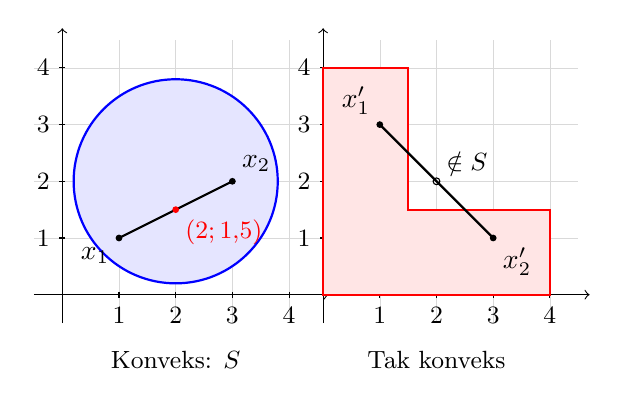
\begin{tikzpicture}[scale=0.72]
  \begin{scope}
    \draw[help lines, gray!30] (-0.5,-0.5) grid (4.5,4.5);
    \draw[->, thin] (-0.5,0) -- (4.7,0);
    \draw[->, thin] (0,-0.5) -- (0,4.7);
    \foreach \i in {1,2,3,4} {
      \draw (\i,0.05) -- (\i,-0.05) node[below] {\small \i};
      \draw (0.05,\i) -- (-0.05,\i) node[left] {\small \i};
    }
    \draw[thick, blue, fill=blue!10] (2,2) circle (1.8);
    \fill (1,1) circle (1.7pt) node[below left] {$x_1$};
    \fill (3,2) circle (1.7pt) node[above right] {$x_2$};
    \draw[thick] (1,1) -- (3,2);
    \fill[red] (2,1.5) circle (1.7pt)
      node[below right] {\small $(2;1{,}5)$};
    \node at (2,-1.15) {\small Konveks: $S$};
  \end{scope}

  \begin{scope}[xshift=4.6cm]
    \draw[help lines, gray!30] (-0.5,-0.5) grid (4.5,4.5);
    \draw[->, thin] (-0.5,0) -- (4.7,0);
    \draw[->, thin] (0,-0.5) -- (0,4.7);
    \foreach \i in {1,2,3,4} {
      \draw (\i,0.05) -- (\i,-0.05) node[below] {\small \i};
      \draw (0.05,\i) -- (-0.05,\i) node[left] {\small \i};
    }
    \draw[thick, red, fill=red!10]
      (0,0) -- (4,0) -- (4,1.5) -- (1.5,1.5)
      -- (1.5,4) -- (0,4) -- cycle;
    \fill (1,3) circle (1.7pt) node[above left] {$x_1'$};
    \fill (3,1) circle (1.7pt) node[below right] {$x_2'$};
    \draw[thick] (1,3) -- (3,1);
    \draw (2,2) circle (1.7pt);
    \node[above right] at (2,2) {\small $\notin S$};
    \node at (2,-1.15) {\small Tak konveks};
  \end{scope}
\end{tikzpicture}
\caption{Contoh himpunan konveks (kiri) dan tak konveks (kanan).
Pada himpunan tak konveks, ruas garis antara $x_1'$ dan $x_2'$
melewati titik $(2,2)$ yang berada di luar himpunan.}
\label{fig:konveks}
\end{figure}


\subsection{Kombinasi Konveks dan Convex Hull}
\label{subsec:kombinasikonveks}

Konsep himpunan konveks dapat diperluas untuk mencampurkan lebih dari
dua titik. Campuran ini disebut \textit{kombinasi konveks} apabila
setiap bobot tidak negatif dan jumlah seluruh bobotnya sama dengan
satu.

\begin{definisi}[\citealp{boyd}]
\label{def:kombinasikonveks}
Untuk titik-titik $x_1,\dots,x_k\in\mathbb{R}^n$ dan skalar
$\theta_1,\dots,\theta_k$ yang memenuhi
$\theta_i\geq 0$ dan $\sum_{i=1}^{k}\theta_i=1$, titik
\begin{equation}
    \sum_{i=1}^{k}\theta_i x_i
    \label{eq:kombinasikonveks}
\end{equation}
disebut \textit{kombinasi konveks} dari $x_1,\dots,x_k$.
\end{definisi}

Kumpulan seluruh kombinasi konveks dari titik-titik dalam suatu
himpunan membentuk \textit{convex hull}, yaitu himpunan konveks
terkecil yang memuat himpunan tersebut.

\begin{definisi}[\citealp{boyd}]
\label{def:convexhull}
\textit{Convex hull} dari himpunan $S\subseteq\mathbb{R}^n$,
ditulis $\operatorname{conv}(S)$, didefinisikan sebagai
\begin{equation}
    \operatorname{conv}(S)
    =
    \left\{
    \sum_{i=1}^{k}\theta_i x_i
    \;\middle|\;
    \begin{array}{l}
    k\in\mathbb{N},\ x_i\in S,\ \theta_i\geq 0,\\
    \displaystyle\sum_{i=1}^{k}\theta_i=1
    \end{array}
    \right\},
    \label{eq:convexhull}
\end{equation}
sehingga $\operatorname{conv}(S)$ merupakan himpunan
konveks terkecil yang memuat $S$.
\end{definisi}


\subsection{Simpleks Probabilitas}
\label{subsec:simpleksprobabilitas}

Salah satu contoh penting yang berkaitan dengan kombinasi konveks
adalah \textit{simpleks probabilitas}, yaitu himpunan seluruh vektor
probabilitas untuk $V$ kategori. Setiap komponennya tidak negatif
dan jumlah seluruh komponennya sama dengan satu.

\begin{definisi}[\citealp{boyd}]
\label{def:simpleks}
\textit{Simpleks probabilitas} berdimensi $V-1$ didefinisikan sebagai
\begin{equation}
    \Delta^{V-1}
    =
    \left\{
    p=(p_1,\dots,p_V)^\top\in\mathbb{R}^{V}
    \;\middle|\;
    p_i\geq 0,\ 
    \sum_{i=1}^{V}p_i=1
    \right\}.
    \label{eq:simpleks}
\end{equation}
\end{definisi}

Simpleks probabilitas merupakan \textit{convex hull} dari vektor
indikator $e_1,\dots,e_V$ (Definisi~\ref{def:onehot}), yaitu
\begin{equation}
    \Delta^{V-1}
    =
    \operatorname{conv}\{e_1,\dots,e_V\}.
\end{equation}
Setiap vektor probabilitas $p\in\Delta^{V-1}$ dapat dinyatakan
sebagai kombinasi konveks
\begin{equation}
    p=\sum_{i=1}^{V}p_i e_i.
\end{equation}
Dalam representasi ini, setiap vektor indikator merupakan titik
sudut simpleks yang menyatakan probabilitas satu pada satu kategori,
sedangkan titik-titik lainnya menyatakan distribusi probabilitas
yang tersebar di antara beberapa kategori.

Gambar~\ref{fig:simpleks} mengilustrasikan simpleks probabilitas
untuk $V=3$ kategori. Karena $p_1+p_2+p_3=1$, simpleks tersebut
dapat digambarkan pada bidang $(p_1,p_2)$ dengan
$p_3=1-p_1-p_2$.

\begin{figure}[H]
\centering
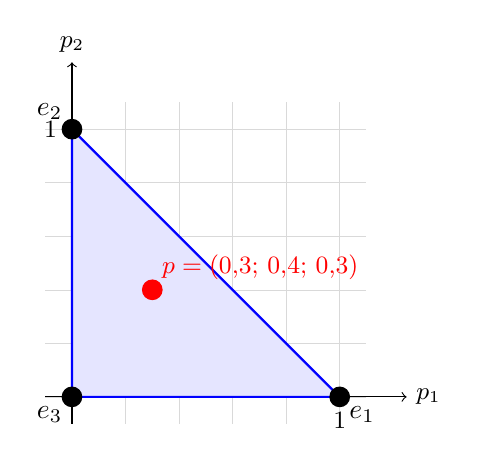
\begin{tikzpicture}[scale=3.4]
  \draw[help lines, gray!30, step=0.2] (-0.1,-0.1) grid (1.1,1.1);
  \draw[->, thin] (-0.1,0) -- (1.25,0) node[right] {\small $p_1$};
  \draw[->, thin] (0,-0.1) -- (0,1.25) node[above] {\small $p_2$};
  \draw (1,0.02) -- (1,-0.02) node[below] {\small $1$};
  \draw (0.02,1) -- (-0.02,1) node[left] {\small $1$};

  \draw[thick, blue, fill=blue!10] (1,0) -- (0,1) -- (0,0) -- cycle;
  \fill (1,0) circle (1.1pt) node[below right] {$e_1$};
  \fill (0,1) circle (1.1pt) node[above left] {$e_2$};
  \fill (0,0) circle (1.1pt) node[below left] {$e_3$};
  \fill[red] (0.3,0.4) circle (1.1pt)
    node[above right] {\small $p=(0{,}3;\,0{,}4;\,0{,}3)$};
\end{tikzpicture}
\caption{Simpleks probabilitas $\Delta^2$ untuk $V=3$ kategori
pada bidang $(p_1,p_2)$. Titik sudut $e_1,e_2,e_3$ menyatakan
distribusi yang pasti pada satu kategori, sedangkan titik di bagian
dalam menyatakan distribusi campuran.}
\label{fig:simpleks}
\end{figure}



\section{Entropi}
\label{sec:entropi}

\subsection{Entropi Shannon}
\label{subsec:entropishannon}

Entropi Shannon mengukur ketidakpastian suatu variabel random
diskret. Misalkan $X$ merupakan variabel random diskret dengan
ruang nilai $\mathcal{X}$ dan fungsi massa probabilitas $p(x)$.
Entropi Shannon didefinisikan sebagai berikut.

\begin{definisi}[\citealp{cover}]
\label{def:entropishannon}
Entropi Shannon dari variabel random diskret $X$ adalah
\begin{equation}
    H(X)=-\sum_{x\in\mathcal{X}}p(x)\log p(x),
    \label{eq:entropishannon}
\end{equation}
dengan konvensi $0\log 0:=0$.
\end{definisi}

\subsection{Batas Entropi}
\label{subsec:batasentropi}

Untuk variabel random diskret $X$ dengan ruang nilai berhingga
$\mathcal{X}$, entropi Shannon memenuhi batas berikut
\citep{cover}.

\begin{equation}
    0\leq H(X)\leq\log|\mathcal{X}|.
    \label{eq:batasentropi}
\end{equation}

Batas bawah dicapai jika dan hanya jika distribusi probabilitas
$X$ terkonsentrasi pada satu nilai, sedangkan batas atas dicapai
jika dan hanya jika distribusi probabilitas $X$ seragam pada
$\mathcal{X}$.


\section{Inferensi Bayes}
\label{sec:bayes}

Inferensi Bayes merupakan pendekatan untuk melakukan inferensi terhadap
parameter yang tidak diketahui dengan menggabungkan informasi awal
mengenai parameter dan informasi yang diperoleh dari data. Informasi
awal dinyatakan melalui distribusi prior, sedangkan informasi dari data
dinyatakan melalui likelihood. Penggabungan keduanya menghasilkan
distribusi posterior yang menggambarkan ketidakpastian parameter setelah
data diamati \citep{casella}.

\subsection{Definisi Bayes: Prior, Likelihood, dan Posterior}
\label{subsec:definisibayes}

\begin{definisi}[Rumus Bayes; \citealp{casella}]
\label{def:bayes}
Misalkan $\theta$ merupakan parameter dan $Y$ merupakan variabel random
yang menghasilkan data $y$. Jika $f(\theta)$ merupakan distribusi prior
dan $f(y\mid\theta)$ merupakan fungsi massa peluang atau fungsi kepadatan
bersyarat dari $Y$ diberikan $\theta$, maka distribusi posterior
$\theta$ setelah data $y$ diamati adalah
\begin{equation}
f(\theta\mid y)
=
\frac{f(y\mid\theta)f(\theta)}{f(y)}.
\label{eq:bayes}
\end{equation}
Untuk parameter kontinu, evidence $f(y)$ diperoleh melalui
\begin{equation}
f(y)
=
\int f(y\mid\theta)f(\theta)\,d\theta.
\label{eq:evidencekontinu}
\end{equation}
Untuk parameter diskret, integral digantikan dengan penjumlahan.
\end{definisi}

Pada Persamaan~\eqref{eq:bayes}, $f(\theta)$ merupakan prior,
$f(y\mid\theta)$ merupakan likelihood, $f(y)$ merupakan evidence,
dan $f(\theta\mid y)$ merupakan posterior. Evidence berfungsi sebagai
konstanta normalisasi agar posterior merupakan distribusi probabilitas
yang sah. Karena evidence tidak bergantung pada $\theta$, posterior
juga dapat dinyatakan secara proporsional sebagai
\begin{equation}
f(\theta\mid y)
\propto f(y\mid\theta)f(\theta).
\label{eq:bayesproporsional}
\end{equation}
Bentuk proporsional ini memudahkan penentuan posterior ketika hasil
perkalian likelihood dan prior sudah dapat dikenali sebagai kernel
suatu keluarga distribusi.


\subsection{Prior Konjugat}
\label{subsec:priorkonjugat}

\begin{definisi}[\citealp{casella}]
\label{def:priorkonjugat}
Keluarga distribusi prior $\mathcal{F}$ disebut konjugat terhadap
likelihood $f(y\mid\theta)$ apabila posterior yang diperoleh dari
setiap prior dalam $\mathcal{F}$ juga termasuk dalam keluarga
distribusi $\mathcal{F}$.
\end{definisi}

Kekonjugatan memungkinkan posterior dinyatakan dalam bentuk tertutup
tanpa harus menghitung evidence secara eksplisit. Salah satu contoh
yang relevan dalam penelitian ini adalah kekonjugatan Dirichlet--Multinomial.


\subsection{Kekonjugatan Dirichlet--Multinomial}
\label{subsec:konjugasidirichletmultinomial}

\begin{definisi}[\citealp{gelman}]
\label{def:konjugasidirichletmultinomial}
Misalkan vektor probabilitas
$\theta=(\theta_1,\ldots,\theta_V)^\top$ memiliki prior
\[
\theta\sim\operatorname{Dir}(\alpha),
\qquad
\alpha=(\alpha_1,\ldots,\alpha_V)^\top,
\]
dengan $\alpha_i>0$. Jika, diberikan $\theta$, vektor frekuensi
kategori $\bm{c}=(c_1,\ldots,c_V)^\top$ mengikuti distribusi
Multinomial dengan ukuran sampel $n$, maka posteriornya adalah
\begin{equation}
\theta\mid\bm{c}
\sim\operatorname{Dir}(\alpha+\bm{c}).
\label{eq:konjugasidirichletmultinomial}
\end{equation}
\end{definisi}

Hasil tersebut dapat diturunkan menggunakan Rumus Bayes dengan
mengalikan likelihood Multinomial dan prior Dirichlet. Berdasarkan
Persamaan~\eqref{eq:multinomial}, fungsi likelihood untuk vektor
frekuensi $\bm{c}$ adalah
\begin{equation}
f(\bm{c}\mid\theta)
=
\frac{n!}{\prod_{i=1}^{V}c_i!}
\prod_{i=1}^{V}\theta_i^{c_i},
\label{eq:likelihoodmultinomial}
\end{equation}
dengan $\sum_{i=1}^{V}c_i=n$. Sementara itu, berdasarkan
Persamaan~\eqref{eq:dirichlet}, fungsi kepadatan prior Dirichlet
adalah
\begin{equation}
f(\theta)
=
\frac{1}{B(\alpha)}
\prod_{i=1}^{V}\theta_i^{\alpha_i-1},
\label{eq:priorlengkap}
\end{equation}
dengan $B(\alpha)$ merupakan konstanta normalisasi distribusi
Dirichlet.

Menurut Rumus Bayes pada Persamaan~\eqref{eq:bayes}, posterior
sebanding dengan perkalian likelihood dan prior. Oleh karena itu,
diperoleh
\begin{align}
f(\theta\mid\bm{c})
&\propto f(\bm{c}\mid\theta)f(\theta)
\nonumber\\
&=
\frac{n!}{\prod_{i=1}^{V}c_i!}
\frac{1}{B(\alpha)}
\left(\prod_{i=1}^{V}\theta_i^{c_i}\right)
\left(\prod_{i=1}^{V}\theta_i^{\alpha_i-1}\right).
\label{eq:perkalianlikelihoodprior}
\end{align}

Pada Persamaan~\eqref{eq:perkalianlikelihoodprior}, faktor
$\frac{n!}{\prod_{i=1}^{V}c_i!}$ dan $\frac{1}{B(\alpha)}$
tidak bergantung pada $\theta$. Karena itu, kedua faktor tersebut
dapat diserap ke dalam konstanta proporsionalitas. Selanjutnya,
menggunakan sifat perkalian berpangkat
$x^a x^b=x^{a+b}$, diperoleh
\begin{align}
f(\theta\mid\bm{c})
&\propto
\prod_{i=1}^{V}
\theta_i^{c_i}\theta_i^{\alpha_i-1}
\nonumber\\
&=
\prod_{i=1}^{V}
\theta_i^{\alpha_i+c_i-1}.
\label{eq:kernelposterior}
\end{align}

Bentuk pada Persamaan~\eqref{eq:kernelposterior} sama dengan
bentuk kernel distribusi Dirichlet, yaitu hasil kali setiap
komponen probabilitas yang dipangkatkan dengan parameter
distribusinya dikurangi satu. Dengan membandingkannya dengan
fungsi kepadatan Dirichlet, parameter posterior dapat diidentifikasi
sebagai $\alpha_i+c_i$ untuk setiap kategori $i$.

Agar menjadi fungsi kepadatan probabilitas, kernel
tersebut harus dinormalisasi. Konstanta normalisasinya adalah
$B(\alpha+\bm{c})$, sehingga posterior lengkapnya menjadi
\begin{equation}
f(\theta\mid\bm{c})
=
\frac{1}{B(\alpha+\bm{c})}
\prod_{i=1}^{V}
\theta_i^{\alpha_i+c_i-1}
\label{eq:posteriorlengkap}
\end{equation}
dan diperoleh
$\theta\mid\bm{c}\sim\operatorname{Dir}(\alpha+\bm{c})$,
sebagaimana dinyatakan pada
Persamaan~\eqref{eq:konjugasidirichletmultinomial}. Hasil ini
menunjukkan bahwa keluarga prior Dirichlet tetap menjadi keluarga
posterior setelah pengamatan mengikuti likelihood Multinomial.


Secara intuitif, pembaruan posterior menambahkan frekuensi
pengamatan $c_i$ pada parameter prior $\alpha_i$. Untuk satu
pengamatan pada kategori $y$, vektor frekuensinya merupakan
vektor indikator $e_y$, yang didefinisikan sebagai
\[
(e_y)_i=
\begin{cases}
1, & i=y,\\
0, & i\neq y.
\end{cases}
\]
Oleh karena itu, pembaruan posterior untuk satu pengamatan adalah
\begin{equation}
\theta\mid y
\sim\operatorname{Dir}(\alpha+e_y).
\label{eq:posterioronehot}
\end{equation}
Artinya, parameter prior untuk kategori yang diamati bertambah
satu, sedangkan parameter kategori lainnya tidak berubah.

\begin{definisi}[\citealp{gelman}]
\label{def:pseudocount}
Parameter prior $\alpha_i$ disebut \textit{pseudo-count} kategori
$i$, sedangkan
\[
\alpha_0=\sum_{i=1}^{V}\alpha_i
\]
disebut massa konsentrasi prior. Pembaruan
$\alpha_i\mapsto\alpha_i+c_i$ menambahkan frekuensi pengamatan
kategori $i$ pada pseudo-count kategori tersebut.
\end{definisi}

Berdasarkan rumus ekspektasi distribusi Dirichlet pada
Persamaan~\eqref{eq:ekspektasidirichlet}, ekspektasi komponen
posterior diperoleh dengan mengganti parameter prior
$\alpha_i$ menjadi parameter posterior $\alpha_i+c_i$:
\begin{align}
\mathbb{E}[\theta_i\mid\bm{c}]
&=
\frac{\alpha_i+c_i}
{\sum_{j=1}^{V}(\alpha_j+c_j)}
\nonumber\\
&=
\frac{\alpha_i+c_i}{\alpha_0+n},
\qquad i=1,\ldots,V,
\label{eq:ekspektasiposterior}
\end{align}
karena $\sum_{i=1}^{V}c_i=n$. Persamaan ini menunjukkan bahwa
rerata posterior ditentukan oleh pseudo-count awal dan frekuensi
pengamatan, sedangkan penyebutnya merupakan total konsentrasi
setelah pembaruan.

\subsection{Rerata Posterior sebagai Estimator Bayes}
\label{subsec:estimatorbayes}

\begin{definisi}[\citealp{casella}]
\label{def:risikokuadratik}
Misalkan $\theta\in\mathbb{R}^{V}$ merupakan parameter random
dan $\delta=\delta(y)\in\mathbb{R}^{V}$ merupakan penduga
parameter berdasarkan data $y$. Risiko posterior dengan \textit{squared loss} didefinisikan sebagai
\begin{equation}
R(\delta\mid y)
=
\mathbb{E}\left[
\lVert\theta-\delta\rVert_2^2
\mid y
\right].
\label{eq:risikokuadratik}
\end{equation}
Penduga yang meminimumkan risiko posterior tersebut disebut
estimator Bayes di bawah \textit{squared loss}.
\end{definisi}

Untuk menunjukkan bahwa rerata posterior merupakan estimator
Bayes di bawah \textit{squared loss}, definisikan
$\mu_i=\mathbb{E}[\theta_i\mid y]$. Karena kuadrat norma
Euclidean merupakan jumlah kuadrat setiap komponen, risiko
posterior dapat dituliskan sebagai
\begin{align}
R(\delta\mid y)
&=
\mathbb{E}\left[
\sum_{i=1}^{V}(\theta_i-\delta_i)^2
\mid y
\right]
\nonumber\\
&=
\sum_{i=1}^{V}
\mathbb{E}\left[
(\theta_i-\delta_i)^2\mid y
\right].
\label{eq:risikokomponen}
\end{align}
Langkah kedua menggunakan linearitas ekspektasi, yaitu
ekspektasi dari jumlah berhingga sama dengan jumlah ekspektasi
masing-masing suku.

Selanjutnya, setiap selisih $\theta_i-\delta_i$ dapat diuraikan
dengan menambahkan dan mengurangkan rerata posterior $\mu_i$:
\begin{equation}
\theta_i-\delta_i
=
(\theta_i-\mu_i)+(\mu_i-\delta_i).
\label{eq:uraianselisih}
\end{equation}
Dengan menguadratkan kedua ruas, diperoleh
\begin{align}
(\theta_i-\delta_i)^2
&=
(\theta_i-\mu_i)^2
+2(\theta_i-\mu_i)(\mu_i-\delta_i)
\nonumber\\
&\quad
+(\mu_i-\delta_i)^2.
\label{eq:kuadratselisih}
\end{align}
Mengambil ekspektasi bersyarat pada data $y$ menghasilkan
\begin{align}
&\mathbb{E}\left[
(\theta_i-\delta_i)^2\mid y
\right]
\nonumber\\
&=
\mathbb{E}\left[
(\theta_i-\mu_i)^2\mid y
\right]
\nonumber\\
&\quad+
2(\mu_i-\delta_i)
\mathbb{E}\left[
\theta_i-\mu_i\mid y
\right]
+(\mu_i-\delta_i)^2.
\label{eq:ekspektasikuadrat}
\end{align}
Pada langkah ini, $\mu_i$ dan $\delta_i$ diperlakukan sebagai
konstanta karena keduanya ditentukan oleh distribusi posterior
setelah data $y$ diamati.

Berdasarkan definisi rerata posterior,
\begin{align}
\mathbb{E}\left[
\theta_i-\mu_i\mid y
\right]
&=
\mathbb{E}[\theta_i\mid y]-\mu_i
\nonumber\\
&=\mu_i-\mu_i=0.
\label{eq:rerataterpusat}
\end{align}
Akibatnya, suku silang pada
Persamaan~\eqref{eq:ekspektasikuadrat} bernilai nol.
Sementara itu, suku pertama merupakan varians posterior karena
$\mu_i=\mathbb{E}[\theta_i\mid y]$. Dengan demikian,
\begin{equation}
\mathbb{E}\left[
(\theta_i-\delta_i)^2\mid y
\right]
=
\operatorname{Var}(\theta_i\mid y)
+(\delta_i-\mu_i)^2.
\label{eq:dekomposisirisiko}
\end{equation}

Substitusi Persamaan~\eqref{eq:dekomposisirisiko} ke dalam
Persamaan~\eqref{eq:risikokomponen} memberikan
\begin{align}
R(\delta\mid y)
&=
\sum_{i=1}^{V}
\operatorname{Var}(\theta_i\mid y)
+
\sum_{i=1}^{V}(\delta_i-\mu_i)^2.
\label{eq:risikoterurai}
\end{align}
Suku pertama tidak bergantung pada penduga $\delta$, sedangkan
suku kedua merupakan jumlah kuadrat yang selalu tidak negatif.
Suku kedua mencapai nilai minimum nol apabila
$\delta_i=\mu_i$ untuk setiap $i$. Oleh karena itu, risiko
posterior minimum dicapai oleh
\begin{equation}
\delta^*
=
\mathbb{E}[\theta\mid y]
=
\begin{pmatrix}
\mathbb{E}[\theta_1\mid y]\\
\vdots\\
\mathbb{E}[\theta_V\mid y]
\end{pmatrix}.
\label{eq:estimatorbayes}
\end{equation}
Rerata posterior merupakan estimator Bayes
di bawah \textit{squared loss}.

Dalam konteks prior Dirichlet dan likelihood Multinomial,
Persamaan~\eqref{eq:ekspektasiposterior} memberikan bentuk
eksplisit estimator Bayes tersebut:
\begin{equation}
\delta_i^*
=
\frac{\alpha_i+c_i}{\alpha_0+n},
\qquad i=1,\ldots,V.
\label{eq:estimatorbayesdirichlet}
\end{equation}
Hasil ini menjadi landasan matematis untuk menggunakan rerata
posterior sebagai bobot campuran dalam metode Mixture of Inputs.



\section{Model Bahasa dan Arsitektur \textit{Transformer}}
\label{sec:transformer}

\subsection{Model Bahasa Autoregresif}
\label{subsec:autoregresif}

\begin{definisi}[\citealp{goodfellow}]
\label{def:modelbahasa}
Misalkan $\mathcal{V}=\{1,\dots,V\}$ kosakata (\textit{vocabulary})
berukuran $V$, dan $x=(x_1,\dots,x_n)$ barisan token dengan $x_t\in
\mathcal{V}$. \textit{Model bahasa} (\textit{language model}) adalah
distribusi peluang atas barisan token, difaktorkan menurut aturan rantai
peluang sebagai
\begin{equation}
  p(x) = \prod_{t=1}^{n} p(x_t \mid x_{<t}),
  \label{eq:autoregresif}
\end{equation}
dengan $x_{<t}=(x_1,\dots,x_{t-1})$. Model yang memfaktorkan peluangnya
demikian --- token ke-$t$ dibangkitkan bergantung pada seluruh token
sebelumnya --- disebut \textit{autoregresif}.
\end{definisi}

Persamaan~\eqref{eq:autoregresif} adalah penerapan berulang aturan rantai
peluang. Untuk $n=3$ misalnya, produknya terurai menjadi tiga faktor,
\begin{equation}
  p(x_1,x_2,x_3) = p(x_1)\,p(x_2\mid x_1)\,p(x_3\mid x_1,x_2),
  \label{eq:autoregresifcontoh}
\end{equation}
dengan $p(x_1)=p(x_1\mid x_{<1})$ memakai $x_{<1}=\varnothing$ (barisan
kosong, tidak ada token sebelum token pertama). Setiap faktor pada
Persamaan~\eqref{eq:autoregresifcontoh} adalah distribusi atas $V$
kategori yang bersyarat pada token-token sebelumnya, sehingga membangkitkan
barisan $x$ berarti membangkitkan token satu per satu secara berurutan:
$x_1$ terlebih dahulu, kemudian $x_2$ dengan $x_1$ diketahui, dan
seterusnya.


\subsection{Jaringan Saraf, Fungsi Aktivasi, dan Fungsi \textit{Softmax}}
\label{subsec:softmax}

Komponen dasar jaringan saraf tiruan adalah lapisan (\textit{layer})
yang memetakan masukan $u\in\mathbb{R}^{m}$ menjadi keluaran
$\sigma(Wu+b)$, dengan $W$ dan $b$ merupakan parameter yang
dipelajari, sedangkan $\sigma$ adalah fungsi aktivasi taklinear,
seperti ReLU atau \textit{tanh}. Fungsi aktivasi memungkinkan
tumpukan lapisan memodelkan hubungan yang lebih kompleks daripada
kombinasi linear semata \citep{goodfellow}. Arsitektur
\textit{Transformer} juga tersusun atas rangkaian lapisan yang
melibatkan operasi linear dan fungsi aktivasi.

Pada model bahasa, lapisan keluaran menghasilkan vektor
\textit{logit} $\ell=(\ell_1,\ldots,\ell_V)^\top\in\mathbb{R}^V$,
dengan setiap $\ell_i$ merupakan skor untuk token ke-$i$ dari
kosakata berukuran $V$. Agar skor tersebut dapat digunakan sebagai
distribusi probabilitas, diperlukan fungsi \textit{softmax}.

\begin{definisi}[\citealp{goodfellow}]
\label{def:softmax}
Fungsi \textit{softmax} memetakan vektor logit
$\ell\in\mathbb{R}^V$ menjadi vektor probabilitas
$p=\operatorname{softmax}(\ell)\in\Delta^{V-1}$, dengan komponen
\begin{equation}
p_i=\frac{\exp(\ell_i)}
{\sum_{j=1}^{V}\exp(\ell_j)},
\qquad i=1,\ldots,V.
\label{eq:softmax}
\end{equation}
Setiap komponen $p_i$ menyatakan probabilitas kategori ke-$i$.
Nilainya positif dan jumlah seluruh komponennya sama dengan satu,
sehingga $p$ merupakan distribusi probabilitas pada simpleks
$\Delta^{V-1}$ (Definisi~\ref{def:simpleks}).
\end{definisi}

Dalam penerapannya, fungsi \textit{softmax} dapat menggunakan
parameter suhu (\textit{temperature}) $T>0$ dengan mengganti logit
$\ell_i$ menjadi $\ell_i/T$:
\begin{equation}
p_i=\frac{\exp(\ell_i/T)}
{\sum_{j=1}^{V}\exp(\ell_j/T)}.
\label{eq:softmax-temperature}
\end{equation}
Parameter $T$ mengatur tingkat ketajaman distribusi. Ketika
$T$ mengecil, perbedaan antarlogit menjadi lebih berpengaruh
sehingga probabilitas cenderung terkonsentrasi pada kategori
dengan logit terbesar. Sebaliknya, ketika $T$ membesar, perbedaan
tersebut semakin berkurang dan distribusi mendekati seragam.

Gambar~\ref{fig:softmax} mengilustrasikan pengaruh suhu terhadap
bentuk distribusi.

\begin{figure}[H]
\centering
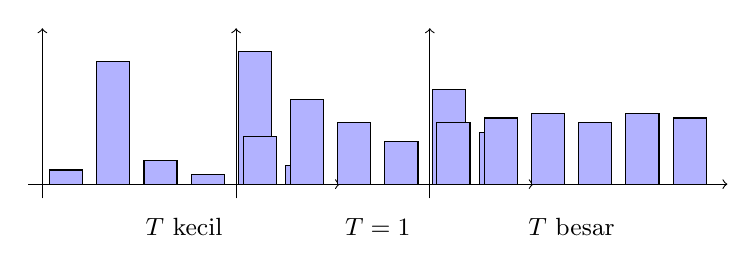
\begin{tikzpicture}[scale=0.6]
  \begin{scope}
    \draw[->, thin] (-0.3,0) -- (6.3,0);
    \draw[->, thin] (0,-0.3) -- (0,3.3);
    \foreach \x/\h in {0.5/0.3, 1.5/2.6, 2.5/0.5, 3.5/0.2, 4.5/2.8, 5.5/0.4} {
      \draw[fill=blue!30] (\x-0.35,0) rectangle (\x+0.35,\h);
    }
    \node at (3,-0.9) {\small $T$ kecil};
  \end{scope}

  \begin{scope}[xshift=4.1cm]
    \draw[->, thin] (-0.3,0) -- (6.3,0);
    \draw[->, thin] (0,-0.3) -- (0,3.3);
    \foreach \x/\h in {0.5/1.0, 1.5/1.8, 2.5/1.3, 3.5/0.9, 4.5/2.0, 5.5/1.1} {
      \draw[fill=blue!30] (\x-0.35,0) rectangle (\x+0.35,\h);
    }
    \node at (3,-0.9) {\small $T=1$};
  \end{scope}

  \begin{scope}[xshift=8.2cm]
    \draw[->, thin] (-0.3,0) -- (6.3,0);
    \draw[->, thin] (0,-0.3) -- (0,3.3);
    \foreach \x/\h in {0.5/1.3, 1.5/1.4, 2.5/1.5, 3.5/1.3, 4.5/1.5, 5.5/1.4} {
      \draw[fill=blue!30] (\x-0.35,0) rectangle (\x+0.35,\h);
    }
    \node at (3,-0.9) {\small $T$ besar};
  \end{scope}
\end{tikzpicture}
\caption{Ilustrasi pengaruh suhu $T$ terhadap distribusi
$p=\operatorname{softmax}(\ell/T)$ untuk logit yang sama.
Suhu kecil menghasilkan distribusi yang lebih tajam, sedangkan
suhu besar menghasilkan distribusi yang lebih mendekati seragam.}
\label{fig:softmax}
\end{figure}




\subsection{Mekanisme Atensi dan \textit{KV-Cache}}
\label{subsec:atensi}

\textit{Transformer} memproses representasi token melalui mekanisme
atensi (\textit{attention}), yang memungkinkan representasi setiap
posisi dibentuk dari kombinasi berbobot representasi posisi-posisi
lain yang relevan.

\begin{definisi}[\citealp{vaswani}]
\label{def:atensi}
Untuk matriks \textit{query} (\textit{query}) $Q\in\mathbb{R}^{n\times d_k}$,
\textit{key} (\textit{key}) $K\in\mathbb{R}^{n\times d_k}$, dan nilai
(\textit{value}) $V\in\mathbb{R}^{n\times d_v}$, mekanisme
\textit{atensi produk-titik berskala} (\textit{scaled dot-product
attention}) didefinisikan sebagai
\begin{equation}
\operatorname{Atensi}(Q,K,V)
=
\operatorname{softmax}
\left(\frac{QK^\top}{\sqrt{d_k}}\right)V,
\label{eq:atensi}
\end{equation}
dengan fungsi \textit{softmax} diterapkan pada setiap baris matriks.
\end{definisi}


\paragraph{Perkalian matriks (\textit{MatMul}).}
Operasi pertama menghitung $QK^\top$. Karena
$Q\in\mathbb{R}^{n\times d_k}$ dan
$K^\top\in\mathbb{R}^{d_k\times n}$, hasilnya merupakan matriks
berukuran $n\times n$. Setiap elemennya merupakan hasil kali titik
(\textit{dot product}) antara satu baris $Q$ dan satu baris $K$:
\begin{equation}
(QK^\top)_{ij}
=
\sum_{r=1}^{d_k}Q_{ir}K_{jr}.
\label{eq:atensi-matmul}
\end{equation}
Nilai tersebut mengukur kesesuaian antara \textit{query} pada posisi $i$
dan \textit{key} pada posisi $j$. Dengan demikian, matriks $QK^\top$
memuat skor kesesuaian setiap posisi terhadap seluruh posisi
lainnya.

\paragraph{Penskalaan (\textit{Scale}).}
Skor kesesuaian kemudian dibagi dengan $\sqrt{d_k}$:
\begin{equation}
S=\frac{QK^\top}{\sqrt{d_k}}.
\label{eq:atensi-scale}
\end{equation}
Pembagian ini mengendalikan besarnya skor sebelum fungsi
\textit{softmax} diterapkan. Ketika dimensi $d_k$ membesar,
hasil kali titik cenderung memiliki varians yang lebih besar
dengan asumsi komponen \textit{query} dan \textit{key} memiliki varians yang
terkendali dan tidak berkorelasi. Skor yang terlalu besar dapat
membuat distribusi \textit{softmax} terlalu terkonsentrasi.
Karena itu, faktor $\sqrt{d_k}$ membantu menjaga skala skor
agar proses pembobotan lebih stabil.

\paragraph{Fungsi \textit{softmax}.}
Fungsi \textit{softmax} diterapkan pada setiap baris matriks $S$
untuk mengubah skor kesesuaian menjadi bobot probabilitas:
\begin{equation}
A_{ij}
=
\frac{\exp(S_{ij})}
{\sum_{r=1}^{n}\exp(S_{ir})}.
\label{eq:atensi-softmax}
\end{equation}
Setiap elemen $A_{ij}$ menunjukkan bobot posisi $j$ ketika
representasi posisi $i$ dibentuk. Untuk setiap baris $i$,
berlaku $A_{ij}\geq 0$ dan $\sum_{j=1}^{n}A_{ij}=1$.
Dengan demikian, bobot tersebut dapat digunakan untuk
menggabungkan informasi dari berbagai posisi.

\paragraph{Pembobotan nilai (\textit{MatMul}).}
Operasi terakhir mengalikan matriks bobot $A$ dengan matriks
\textit{value} $V$:
\begin{equation}
O=AV.
\label{eq:atensi-output}
\end{equation}
Karena $A\in\mathbb{R}^{n\times n}$ dan
$V\in\mathbb{R}^{n\times d_v}$, keluaran
$O\in\mathbb{R}^{n\times d_v}$. Setiap baris keluaran merupakan
kombinasi berbobot baris-baris $V$, dengan bobot yang ditentukan
oleh skor kesesuaian pada tahap sebelumnya. Oleh karena itu,
representasi keluaran menggabungkan informasi dari posisi-posisi
yang memperoleh bobot atensi lebih besar.

Dalam praktiknya, operasi atensi dapat dilakukan pada beberapa
\textit{head} dengan proyeksi dan dimensi masing-masing, kemudian
hasilnya digabungkan melalui mekanisme
\textit{multi-head attention}.

Gambar~\ref{fig:atensi} mengilustrasikan urutan operasi tersebut.

\begin{figure}[H]
\centering
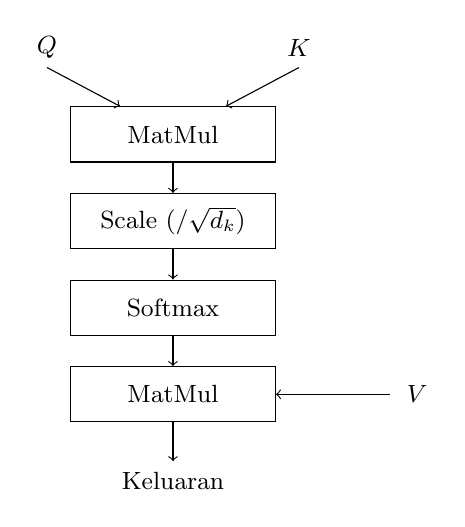
\begin{tikzpicture}[scale=1, every node/.style={font=\small}]
  \node[draw, minimum width=2.6cm, minimum height=0.7cm] (mm1) at (0,0) {MatMul};
  \node[draw, minimum width=2.6cm, minimum height=0.7cm] (sc) at (0,-1.1) {Scale ($/\sqrt{d_k}$)};
  \node[draw, minimum width=2.6cm, minimum height=0.7cm] (sm) at (0,-2.2) {Softmax};
  \node[draw, minimum width=2.6cm, minimum height=0.7cm] (mm2) at (0,-3.3) {MatMul};
  \draw[->] (mm1) -- (sc);
  \draw[->] (sc) -- (sm);
  \draw[->] (sm) -- (mm2);
  \draw[->] (0,-3.65) -- (0,-4.15);
  \node at (0,-4.4) {Keluaran};
  \node at (-1.6,1.1) {$Q$};
  \node at (1.6,1.1) {$K$};
  \draw[->] (-1.6,0.85) -- (mm1);
  \draw[->] (1.6,0.85) -- (mm1);
  \node at (3.1,-3.3) {$V$};
  \draw[->] (2.75,-3.3) -- (mm2);
\end{tikzpicture}
\caption{Alur perhitungan atensi produk-titik berskala pada
Persamaan~\eqref{eq:atensi}, mengikuti diagram \citet{vaswani}.}
\label{fig:atensi}
\end{figure}

Pada pembangkitan teks autoregresif, token dihasilkan satu per
satu. Untuk setiap lapisan, representasi token yang telah diproses
menghasilkan matriks \textit{key} dan \textit{value} yang dapat digunakan kembali
pada langkah berikutnya. Tanpa penyimpanan, model perlu menghitung
ulang \textit{key} dan \textit{value} token-token sebelumnya pada setiap langkah.

\begin{definisi}
\label{def:kvcache}
\textit{KV-cache} pada langkah ke-$t$ menyimpan matriks \textit{key} dan
\textit{value} untuk token-token sebelumnya pada setiap lapisan $l$:
\begin{equation}
\mathcal{M}_t^{(l)}
=
\left\{K_{1:t-1}^{(l)},V_{1:t-1}^{(l)}\right\}.
\label{eq:kvcache}
\end{equation}
Pada langkah $t$, \textit{key} dan \textit{value} token baru dihitung lalu
digabungkan dengan cache yang telah tersimpan. Dengan demikian,
model tidak perlu menghitung ulang \textit{key} dan \textit{value} seluruh
token sebelumnya.
\end{definisi}



\section{Strategi Pengambilan Sampel Token}
\label{sec:sampling}

Setelah distribusi probabilitas token
$p=\operatorname{softmax}(\ell/T)\in\Delta^{V-1}$
diperoleh (Persamaan~\eqref{eq:softmax}), model perlu menentukan
token berikutnya $x_t$ berdasarkan distribusi tersebut. Salah satu
cara adalah \textit{greedy decoding}, yaitu memilih token dengan
probabilitas terbesar,
\begin{equation}
x_t=\operatorname*{arg\,max}_{i\in\mathcal{V}}p_i.
\label{eq:greedy}
\end{equation}
Strategi ini bersifat deterministik untuk distribusi yang sama.
Alternatifnya, model dapat mengambil sampel dari distribusi
kategorik,
\begin{equation}
x_t\sim\operatorname{Kategorik}(p),
\label{eq:categorical-sampling}
\end{equation}
sehingga peluang terpilihnya setiap token sebanding dengan
probabilitasnya. Berbeda dari \textit{greedy decoding}, strategi ini
memungkinkan token dengan probabilitas lebih rendah tetap terpilih.
Namun, sampling langsung dari $p$ juga memungkinkan token dengan
probabilitas sangat kecil terpilih.

Untuk membatasi pilihan token, distribusi probabilitas dapat
dipotong sebelum sampling dilakukan. Dua strategi yang umum
digunakan adalah \textit{top-k sampling} dan \textit{nucleus
sampling} (\textit{top-p sampling}).

\begin{definisi}[\citealp{holtzman}]
\label{def:topk}
Untuk $k\in\{1,\ldots,V\}$, misalkan
$\mathcal{I}_k\subseteq\mathcal{V}$ merupakan himpunan $k$ token
dengan probabilitas terbesar. Pada \textit{top-k sampling},
probabilitas token di luar himpunan tersebut dibuat nol, sedangkan
probabilitas token yang tersisa dinormalisasi ulang:
\begin{equation}
\widetilde p_i=
\begin{cases}
\dfrac{p_i}{\sum_{j\in\mathcal{I}_k}p_j},
& i\in\mathcal{I}_k,\\[1.5ex]
0, & i\notin\mathcal{I}_k.
\end{cases}
\label{eq:topk}
\end{equation}
Dengan demikian, hanya $k$ token dengan probabilitas terbesar
yang dapat dipilih.

Pada \textit{nucleus sampling} atau \textit{top-p sampling},
himpunan token yang dipertahankan ditentukan berdasarkan
probabilitas kumulatif. Misalkan token diurutkan berdasarkan
probabilitas yang menurun. Himpunan $\mathcal{I}_p$ merupakan
himpunan terkecil yang memenuhi
\begin{equation}
\sum_{i\in\mathcal{I}_p}p_i\geq p,
\qquad p\in(0,1).
\label{eq:nucleus}
\end{equation}
Sama seperti pada \textit{top-k sampling}, probabilitas token
di luar $\mathcal{I}_p$ dibuat nol dan probabilitas token yang
tersisa dinormalisasi ulang sebelum sampling dilakukan.
Perbedaannya, \textit{top-k sampling} membatasi banyaknya token,
sedangkan \textit{top-p sampling} membatasi massa probabilitas
kumulatif yang dipertahankan.
\end{definisi}

\begin{figure}[H]
\centering
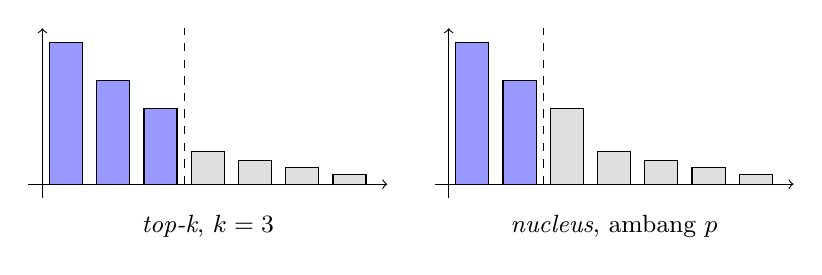
\begin{tikzpicture}[scale=0.6]
  \begin{scope}
    \draw[->, thin] (-0.3,0) -- (7.3,0);
    \draw[->, thin] (0,-0.3) -- (0,3.3);
    \draw[fill=blue!40]  (0.15,0) rectangle (0.85,3.0);
    \draw[fill=blue!40]  (1.15,0) rectangle (1.85,2.2);
    \draw[fill=blue!40]  (2.15,0) rectangle (2.85,1.6);
    \draw[fill=gray!25]  (3.15,0) rectangle (3.85,0.7);
    \draw[fill=gray!25]  (4.15,0) rectangle (4.85,0.5);
    \draw[fill=gray!25]  (5.15,0) rectangle (5.85,0.35);
    \draw[fill=gray!25]  (6.15,0) rectangle (6.85,0.2);
    \draw[dashed] (3.0,0) -- (3.0,3.3);
    \node at (3.5,-0.9) {\small \textit{top-k}, $k=3$};
  \end{scope}

  \begin{scope}[xshift=8.6cm]
    \draw[->, thin] (-0.3,0) -- (7.3,0);
    \draw[->, thin] (0,-0.3) -- (0,3.3);
    \draw[fill=blue!40]  (0.15,0) rectangle (0.85,3.0);
    \draw[fill=blue!40]  (1.15,0) rectangle (1.85,2.2);
    \draw[fill=gray!25]  (2.15,0) rectangle (2.85,1.6);
    \draw[fill=gray!25]  (3.15,0) rectangle (3.85,0.7);
    \draw[fill=gray!25]  (4.15,0) rectangle (4.85,0.5);
    \draw[fill=gray!25]  (5.15,0) rectangle (5.85,0.35);
    \draw[fill=gray!25]  (6.15,0) rectangle (6.85,0.2);
    \draw[dashed] (2.0,0) -- (2.0,3.3);
    \node at (3.5,-0.9) {\small \textit{nucleus}, ambang $p$};
  \end{scope}
\end{tikzpicture}
\caption{Perbandingan \textit{top-k sampling} (kiri, memotong pada
banyaknya kategori) dan \textit{nucleus sampling} (kanan, memotong pada
peluang kumulatif). Batang biru menandai kategori yang tersisa untuk
disampling ulang; batang abu-abu tersisih.}
\label{fig:sampling}
\end{figure}

Gambar~\ref{fig:sampling} mengilustrasikan perbedaan kedua strategi
tersebut. Pada \textit{top-k sampling}, jumlah token yang
dipertahankan ditentukan oleh $k$, sedangkan pada
\textit{top-p sampling}, jumlahnya dapat berubah mengikuti
bentuk distribusi probabilitas.

Dalam penelitian ini, strategi pengambilan token perlu dibedakan
berdasarkan penggunaannya. Pada medium komunikasi teks
(\texttt{text}), setiap agen menghasilkan keluaran teks melalui
proses generasi autoregresif. Implementasi menggunakan sampling
stokastik dengan parameter suhu $T=0{,}6$, \textit{top-k} sebesar
20, dan \textit{top-p} sebesar 0{,}95 sebagai nilai bawaan mesin
generasi. Pada setiap langkah, token berikutnya dipilih berdasarkan
distribusi yang telah dipengaruhi oleh suhu dan pembatasan
sampling tersebut. Proses ini diulang hingga generasi berakhir.
Keluaran teks dari agen perantara kemudian diberikan kepada agen
berikutnya sebagai konteks tekstual. Agen \textit{judger} juga
menggunakan mekanisme generasi teks ini untuk menghasilkan
jawaban akhir.



\section{Sistem Multi-Agen}
\label{sec:multiagen}

\subsection{Definisi Agen dan Sistem Multi-Agen}
\label{subsec:agen}

\begin{definisi}[\citealp{wooldridge2009}]
\label{def:agen}
\textit{Agen} (\textit{agent}) adalah entitas komputasi yang mengamati
lingkungannya melalui sensor dan bertindak terhadap lingkungan itu melalui
aktuator secara otonom --- tanpa campur tangan langsung manusia atau agen
lain pada setiap langkahnya --- untuk mencapai tujuan tertentu.
\end{definisi}

\begin{definisi}[\citealp{wooldridge2009}]
\label{def:mas}
\textit{Sistem multi-agen} (\textit{multi-agent system}, MAS) adalah
sistem yang tersusun atas dua atau lebih agen yang berinteraksi --- saling
bertukar informasi dan saling memengaruhi tindakan satu sama lain --- di
dalam lingkungan bersama.
\end{definisi}

Gambar~\ref{fig:agen} menggambarkan siklus persepsi--tindakan satu agen
terhadap lingkungannya.

\begin{figure}[H]
\centering
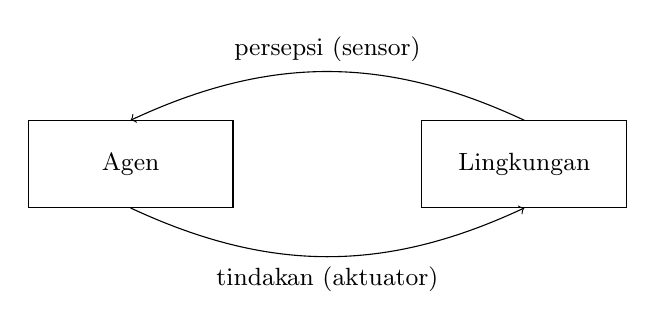
\begin{tikzpicture}[scale=1, every node/.style={font=\small}]
  \node[draw, minimum width=2.6cm, minimum height=1.1cm] (agen) at (0,0) {Agen};
  \node[draw, minimum width=2.6cm, minimum height=1.1cm] (ling) at (5,0) {Lingkungan};
  \draw[->] (ling.north) to[bend right=25] node[above]{persepsi (sensor)} (agen.north);
  \draw[->] (agen.south) to[bend right=25] node[below]{tindakan (aktuator)} (ling.south);
\end{tikzpicture}
\caption{Siklus persepsi--tindakan agen dan lingkungannya
\citep{wooldridge2009}. Pada sistem multi-agen, beberapa agen semacam ini
berbagi satu lingkungan dan dapat saling memengaruhi.}
\label{fig:agen}
\end{figure}

\subsection{Topologi Sekuensial dan Hierarkis}
\label{subsec:topologi}

Interaksi antaragen pada sistem multi-agen dapat diatur menurut berbagai
topologi koordinasi; dua yang paling mendasar adalah sekuensial dan
hierarkis \citep{wooldridge2009}. Pada topologi \textit{sekuensial}, agen
disusun sebagai rantai: keluaran satu agen menjadi masukan agen berikutnya,
sehingga informasi mengalir searah dari agen pertama hingga agen terakhir.
Pada topologi \textit{hierarkis}, satu agen berperan sebagai koordinator
yang mendelegasikan sub-tugas kepada beberapa agen bawahan dan
menggabungkan keluaran mereka. Gambar~\ref{fig:topologi} menggambarkan
kedua topologi tersebut.

\begin{figure}[H]
\centering
\begin{tikzpicture}[scale=1, every node/.style={draw, minimum width=1.3cm, minimum height=0.8cm, font=\small}]
  \node (a1) at (0,0) {$A_1$};
  \node (a2) at (1.8,0) {$A_2$};
  \node (a3) at (3.6,0) {$A_3$};
  \node (a4) at (5.4,0) {$A_4$};
  \draw[->] (a1) -- (a2);
  \draw[->] (a2) -- (a3);
  \draw[->] (a3) -- (a4);
  \node[draw=none] at (2.7,-1.0) {\small Sekuensial};

  \node (b0) at (9.6,0.9) {$A_0$};
  \node (b1) at (8.2,-0.6) {$A_1$};
  \node (b2) at (9.6,-0.6) {$A_2$};
  \node (b3) at (11.0,-0.6) {$A_3$};
  \draw[->] (b0) -- (b1);
  \draw[->] (b0) -- (b2);
  \draw[->] (b0) -- (b3);
  \draw[->] (b1) -- (b0);
  \draw[->] (b2) -- (b0);
  \draw[->] (b3) -- (b0);
  \node[draw=none] at (9.6,-1.6) {\small Hierarkis};
\end{tikzpicture}
\caption{Topologi sekuensial (kiri), rantai agen $A_1\to A_2\to A_3\to
A_4$, dan topologi hierarkis (kanan), koordinator $A_0$ yang
mendelegasikan ke $A_1,A_2,A_3$ dan menggabungkan keluarannya.}
\label{fig:topologi}
\end{figure}
